\chapter[Cronograma]{Cronograma}

Para gerenciamento do projeto estamos utilizando a ferramenta Redmine, com esta ferramenta é possível fazer o gerenciamento do projeto no contexto ágil que é o que está sendo utilizado no Projeto.

\begin{figure}[h]
  \centering
  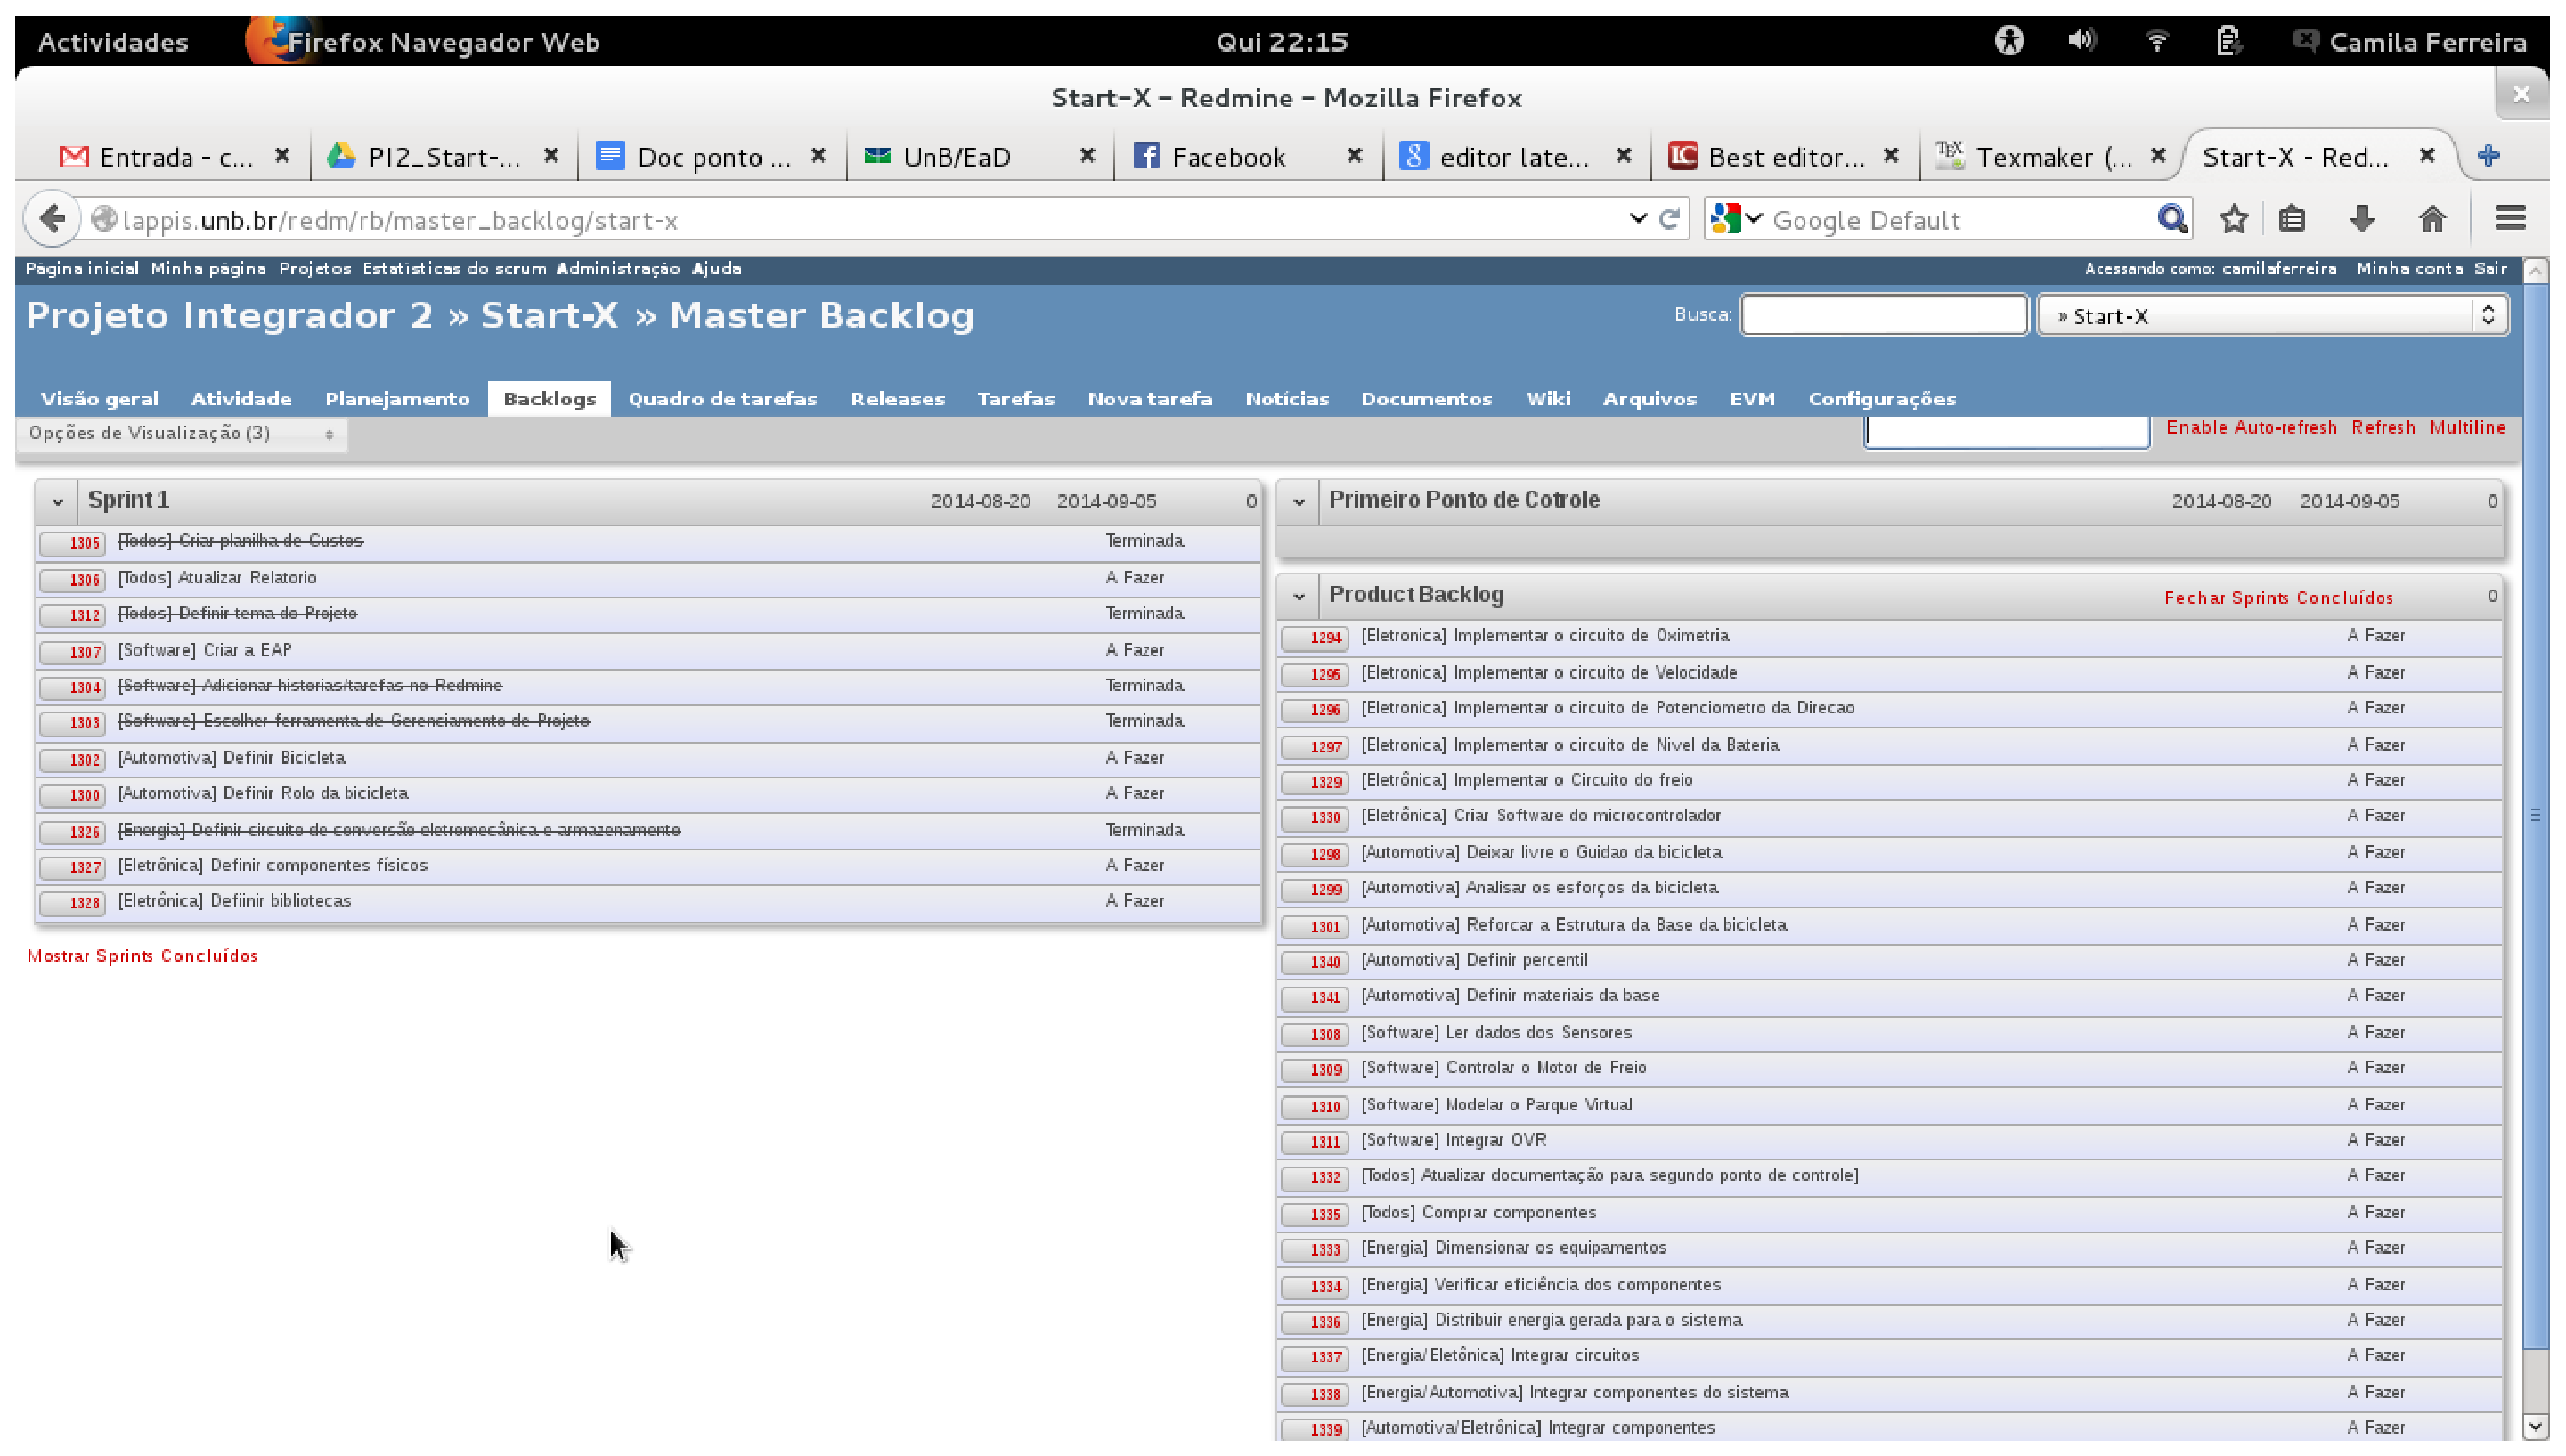
\includegraphics[width=0.8\textwidth]
      {figuras/backlogs.eps}
  \caption[redmine-backlog]
  \label{Redmine e backlog do projeto}
\end{figure}

Para gerir o projeto dividimos o projeto em 3 grandes releases que correspondem com os 3 pontos de controle que teremos duante o semestre. A primeira release se iniciou no primeiro dia de aula de Projeto Integrador 2 e termina no dia do primeiro ponto de controle; a segunda release se iniciará logo após a data do segundo ponto de controle e e terminará no dia do segundo ponto de controle e a terceira relase se iniciará logo após o segundo ponto de controle terminando no dia da entrega final do produto.

\begin{figure}[h]
  \centering
  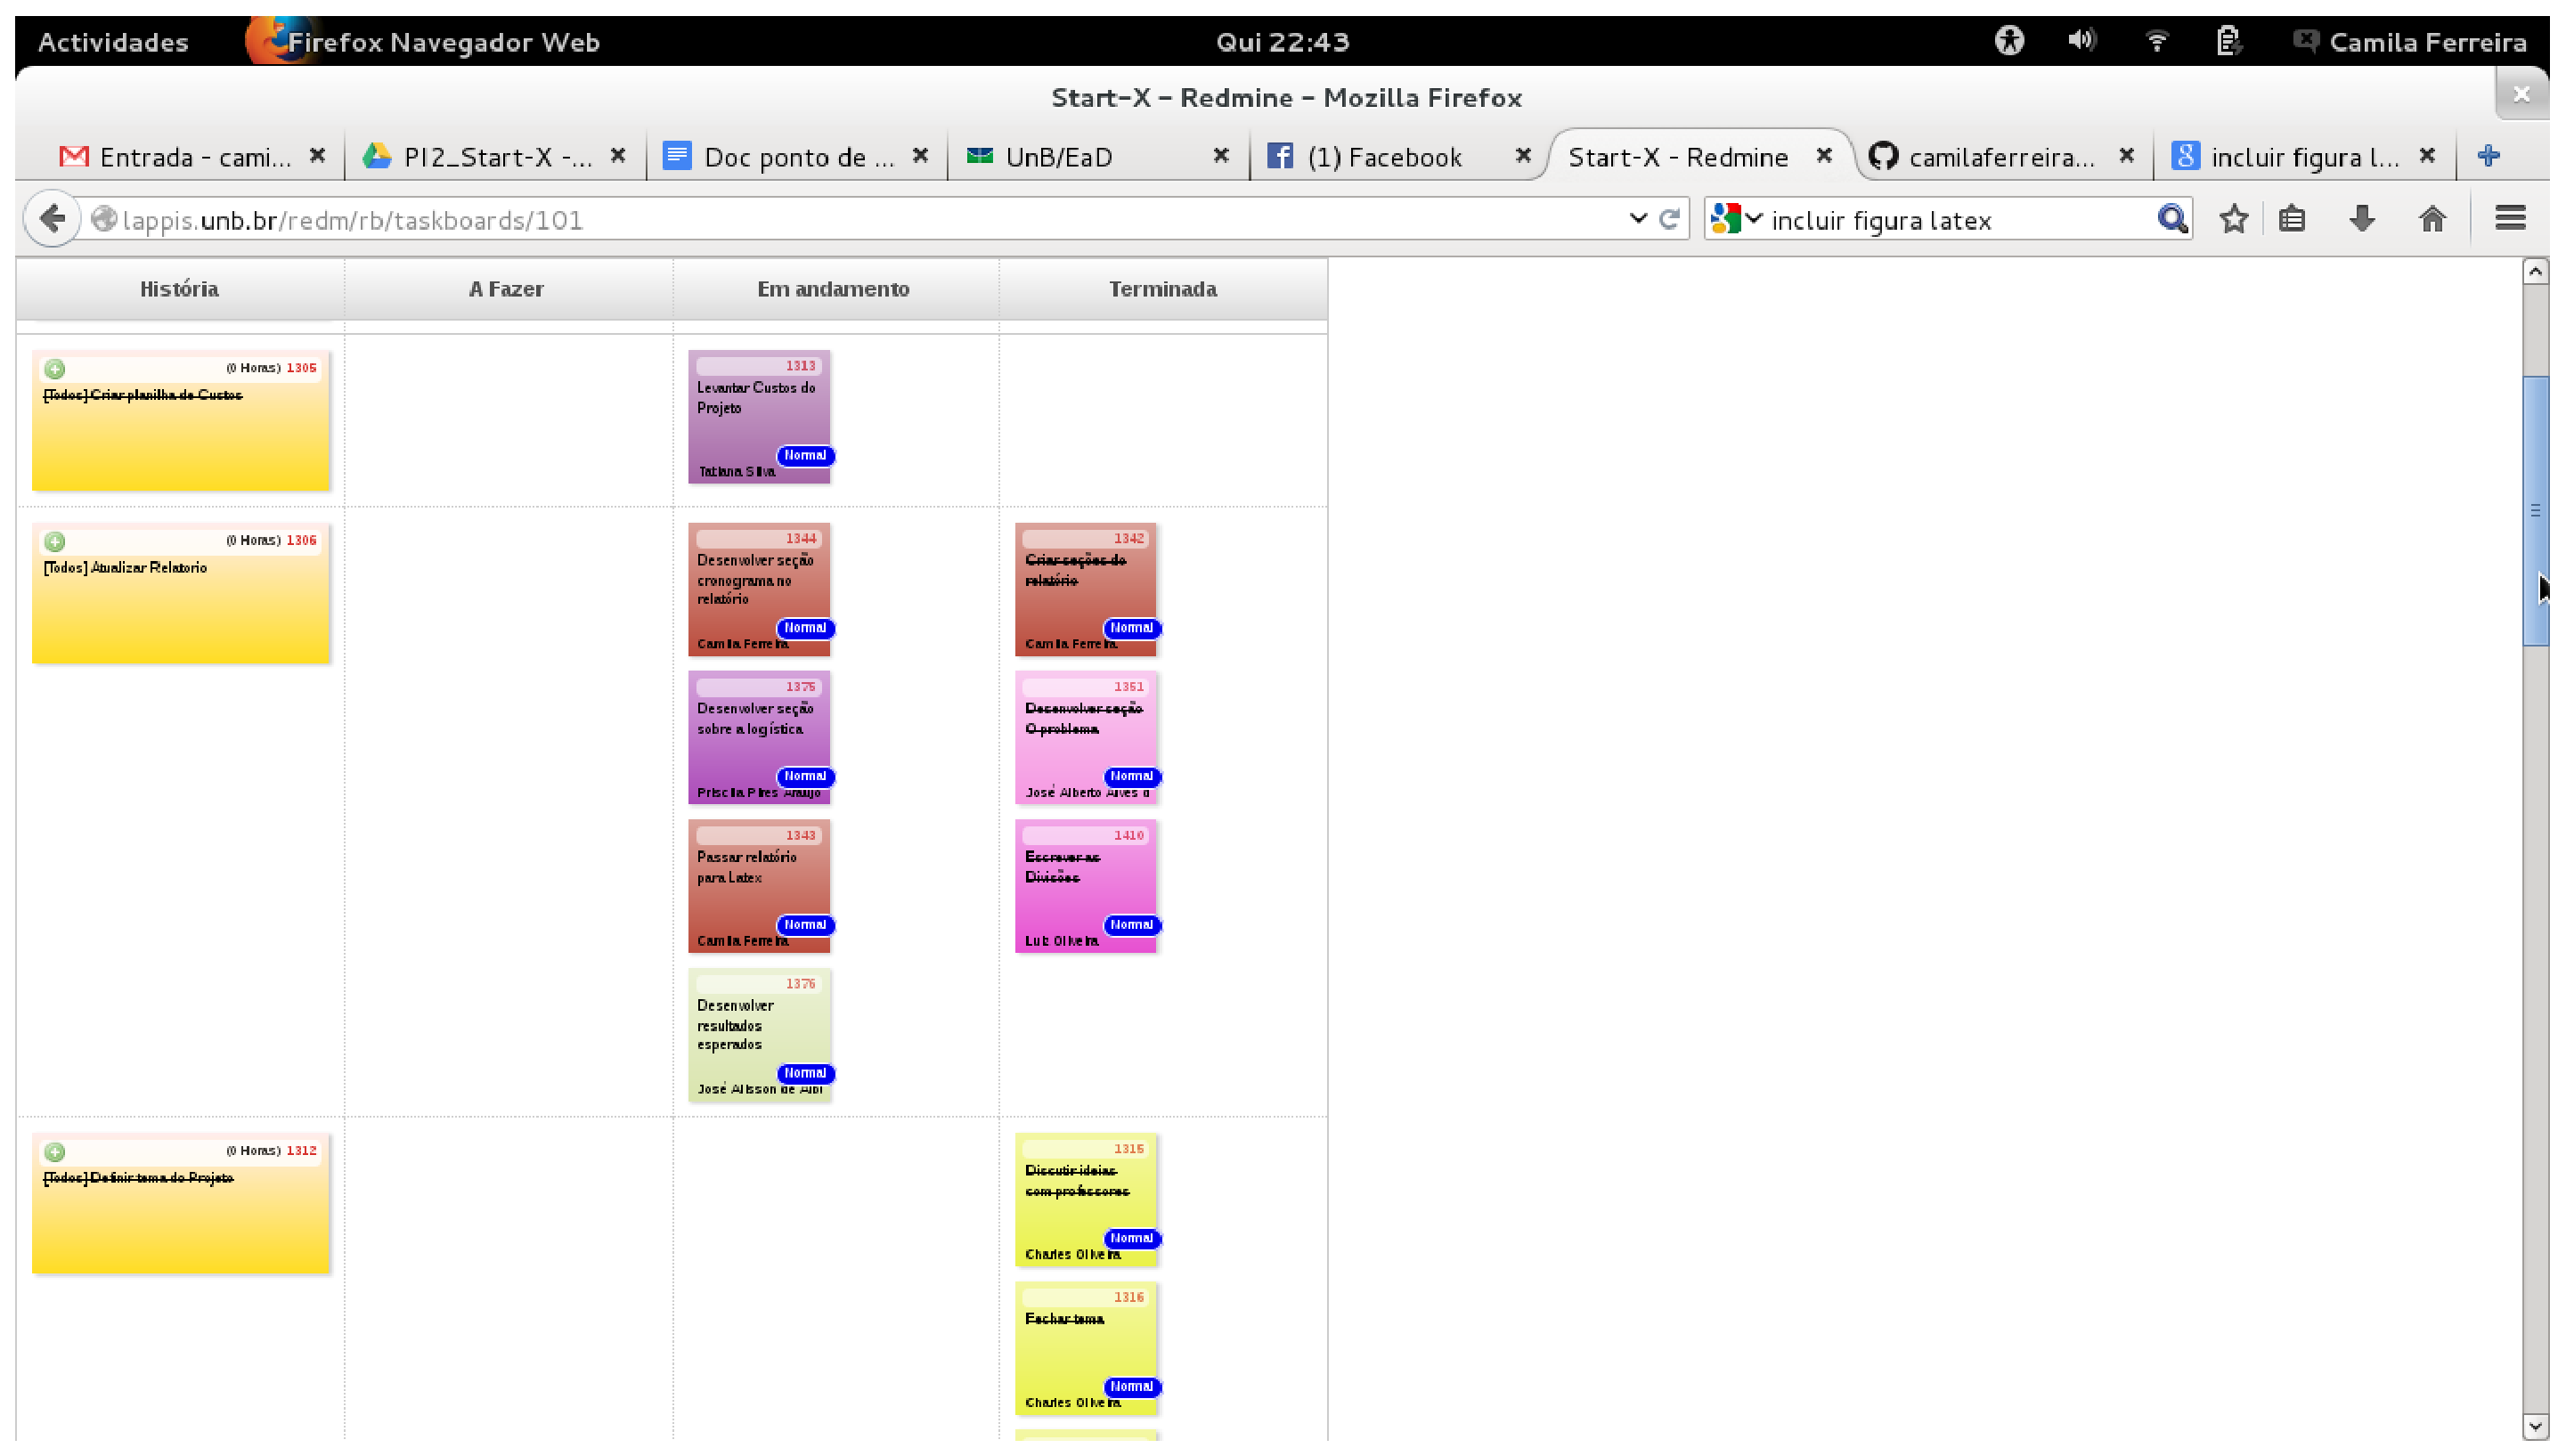
\includegraphics[width=0.8\textwidth]
      {figuras/quadrotarefas.eps}
  \caption[quadro-de-tarefas]
  \label{Quadro de tarefas}
\end{figure}
Para organizar as tarefas do projeto criamos histórias que são macrotarefas onde são posteriormente quebradas em tarefas menores. Essas tarefas são colocadas em um quadro de tarefas.


  
